\documentclass{article}
\usepackage{fancyhdr}
\usepackage{ctex}
\usepackage{listings}
\usepackage{graphicx}
\usepackage[a4paper, body={18cm,22cm}]{geometry}
\usepackage{amsmath,amssymb,amstext,enumerate,graphicx}
\usepackage{float,abstract,booktabs,indentfirst,amsmath}
\usepackage{array}
\usepackage{booktabs}
\usepackage{multirow}
\usepackage{url}
\usepackage{diagbox}
\renewcommand\arraystretch{1.4}
\usepackage{indentfirst}
\setlength{\parindent}{2em}
\usepackage{enumerate}
\setmonofont{Consolas}
\usepackage{listings}
\usepackage{xcolor}
\usepackage{makecell}
\usepackage{enumitem}
\usepackage{tikz}
\usepackage{wrapfig}
\usepackage{tkz-euclide}
\usepackage{pgfplots}
\setfontfamily{\timesfont}{Times New Roman}

\begin{document}

\newcommand{\titem}[1]{
~\\
\begin{itemize}
    \item \heiti \large {#1}
\end{itemize}
}

\newcommand{\bb}[1]{{\heiti {#1}}}

\renewcommand{\d}{\mathrm{d}}

\newcommand{\cf}[1]{$^{#1}\textrm{C}$}

\title{《数学建模及其MATLAB实现》第四次课程作业}
\author{李鹏达}
    

\begin{center}
    \LARGE \textbf{\heiti 《数学建模及其{\timesfont MATLAB}实现》第四次课程作业} \\[0.5em]
    \large 李鹏达 10225101460
\end{center}

\section*{问题1}
某银行经理计划用一笔资金进行有价证券的投资,可供购买的证券以及其信用等级、到期年限、到期税前收益如下表所示。按照规定,市政证券的收益可以免税,其它证券的收益需要缴 $50\%$ 的税额。此外还有以下限制:
\begin{enumerate}
    \item 政府及代办机构的证券总计至少要购买 $400$ 万元;
    \item 所购证券的平均信用等级不超过 $1.4$(信用等级数字越小,信用程度越高);
    \item 所购证券的平均到期年限不超过 $5$ 年。
\end{enumerate}

\subsection*{证券信息表}

\[
\begin{array}{|c|c|c|c|c|}
\hline
\textbf{证券名称} & \textbf{证券种类} & \textbf{信用等级} & \textbf{到期年限} & \textbf{到期税前收益\%} \\
\hline
A & \textrm{市政} & 2 & 9 & 4.3 \\
B & \textrm{代办机构} & 2 & 15 & 5.4 \\
C & \textrm{政府} & 1 & 4 & 5.0 \\
D & \textrm{政府} & 1 & 3 & 4.4 \\
E & \textrm{市政} & 5 & 2 & 4.5 \\
\hline
\end{array}
\]

\subsection*{问题}
\begin{enumerate}
    \item 若该经理有 $1000$ 万元资金,应如何投资?
    \item 如果能够以 $2.75\%$ 的利率借到不超过 $100$ 万元资金,该经理应如何操作?
    \item 在 $1000$ 万元资金情况下,若证券 A 的税前收益增加为 $4.5\%$,投资是否改变?若证券 C 的税前收益减少为 $4.8\%$,投资是否改变?
\end{enumerate}

\subsection*{{\heiti 解答}}

\subsubsection*{1.}

设 $x_A, x_B, x_C, x_D, x_E$ 分别为证券 A, B, C, D, E 的购买金额(万元),设总收益为 $Z$, 则该问题的目标为最大化总收益,即

$$
\max Z = 0.043 x_A + 0.5 \times 0.054 x_B + 0.5 \times 0.05 x_C + 0.5 \times 0.044 x_D + 0.045 x_E
$$

存在的约束条件为:

$$
\text{s.t.} 
\begin{cases}
    x_A + x_B + x_C + x_D + x_E \leq 1000 \quad \text{(资金限制)} \\
    x_B + x_C + x_D \geq 400 \quad \text{(限制1)} \\
    \frac{2 \cdot x_A + 2 \cdot x_B + 1 \cdot x_C + 1 \cdot x_D + 5 \cdot x_E}{x_A + x_B + x_C + x_D + x_E} \leq 1.4 \quad \text{(限制2)} \\
    \frac{9 \cdot x_A + 15 \cdot x_B + 4 \cdot x_C + 3 \cdot x_D + 2 \cdot x_E}{x_A + x_B + x_C + x_D + x_E} \leq 5 \quad \text{(限制3)} \\
    x_A, x_B, x_C, x_D, x_E \geq 0 \quad \text{(非负约束)}
\end{cases}
$$

在 Lingo 中建立模型,求解得到最优解。

\begin{figure}[H]
\centering
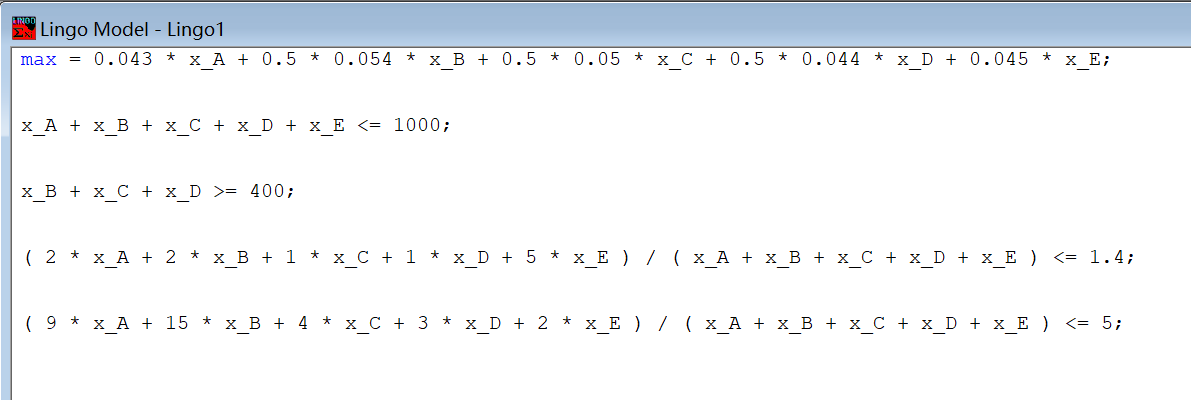
\includegraphics[width=0.7\textwidth]{img/1.png}
\caption{在 Lingo 中建立模型}
\end{figure}

\begin{figure}[H]
\centering
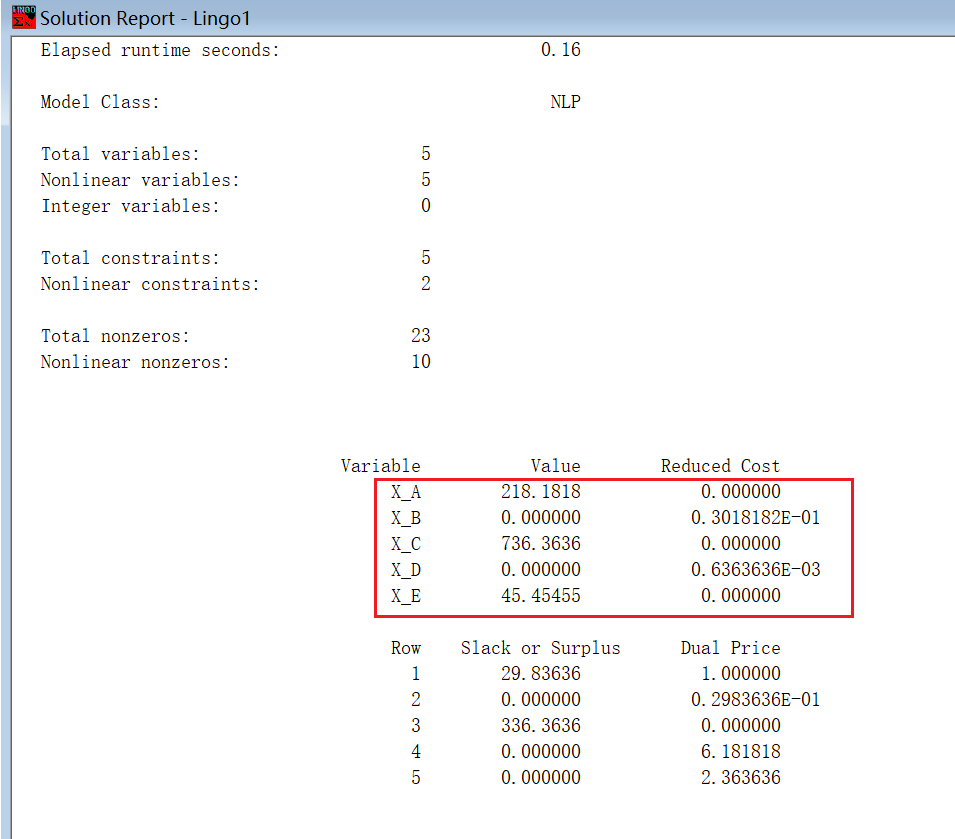
\includegraphics[width=0.5\textwidth]{img/2.png}
\caption{求解得到最优解}
\end{figure}

最优解为

$$
\begin{aligned}
    x_A & = 218.1818 \\
    x_B & = 0.000000 \\
    x_C & = 736.3636 \\
    x_D & = 0.000000 \\
    x_E & = 45.45455 \\
\end{aligned}
$$

\subsubsection*{2.}

如果能够以 2.75\% 的利率借入不超过 100 万元的资金,设借款金额为 \(y\),则总资金为 \(1000 + y\) 万元。此时的目标函数为:
\[
\max Z = (4.3\% \cdot x_A + 5.4\% \cdot 0.5 \cdot x_B + 5.0\% \cdot 0.5 \cdot x_C + 4.4\% \cdot 0.5 \cdot x_D + 4.5\% \cdot x_E) - 2.75\% \cdot y
\]
并且资金约束更新为:
\[
\begin{cases}
    x_A + x_B + x_C + x_D + x_E \leq 1000 + y \\
    0 \leq y \leq 100
\end{cases}
\]

更新 Lingo 模型并求解最优解。

\begin{figure}[H]
\centering
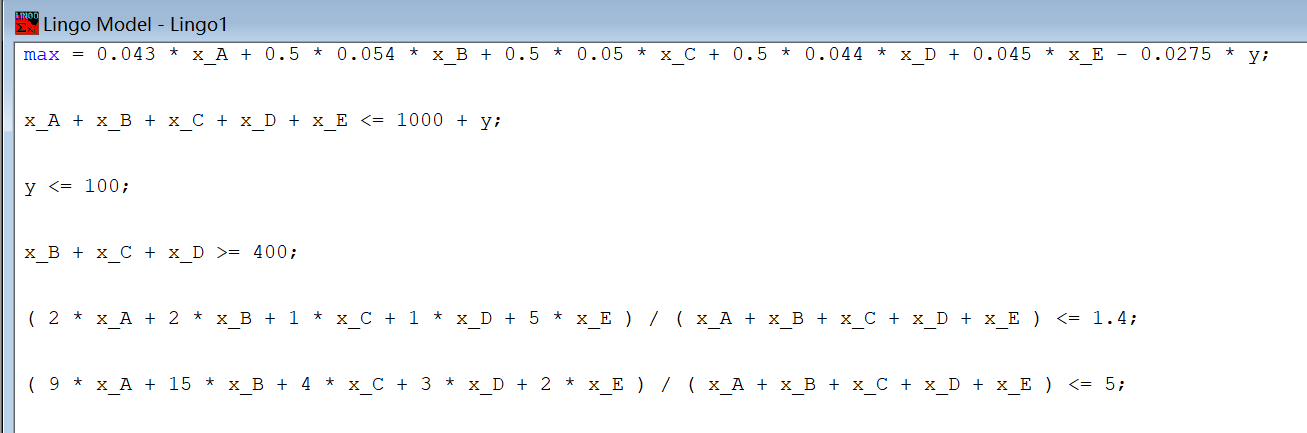
\includegraphics[width=0.9\textwidth]{img/3.png}
\caption{更新后的 Lingo 模型}
\end{figure}

\begin{figure}[H]
\centering
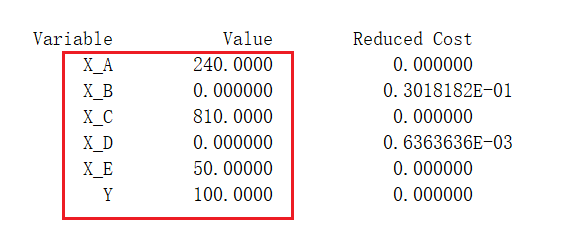
\includegraphics[width=0.5\textwidth]{img/4.png}
\caption{最优解}
\end{figure}

最优解为

\[
\begin{aligned}
    x_A &= 240.0000  \\
    x_B &= 0.000000 \\
    x_C &= 810.0000 \\
    x_D &= 0.000000 \\
    x_E &= 50.00000 \\
      y &= 100.0000 \\
\end{aligned}
\]

\subsection*{3.}
(1) 如果证券 \(A\) 的税前收益增加为 4.5\%,则目标函数变为:
\[
\max Z = 4.5\% \cdot x_A + 5.4\% \cdot 0.5 \cdot x_B + 5.0\% \cdot 0.5 \cdot x_C + 4.4\% \cdot 0.5 \cdot x_D + 4.5\% \cdot x_E
\]

重新求解得到最优解:

\begin{figure}[H]
\centering
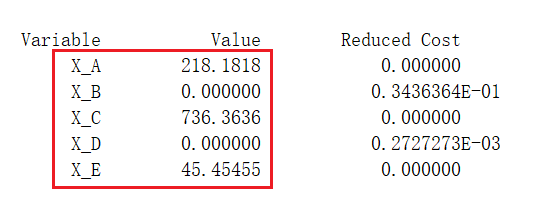
\includegraphics[width=0.7\textwidth]{img/5.png}
\caption{最优解}
\end{figure}

与 1 中的最优解相同,因此投资不改变。

~\\

(2) 如果证券 \(C\) 的税前收益下降为 4.8\%,则目标函数变为:
\[
\max Z = 4.3\% \cdot x_A + 5.4\% \cdot 0.5 \cdot x_B + 4.8\% \cdot 0.5 \cdot x_C + 4.4\% \cdot 0.5 \cdot x_D + 4.5\% \cdot x_E
\]

重新求解得到最优解:

\begin{figure}[H]
\centering
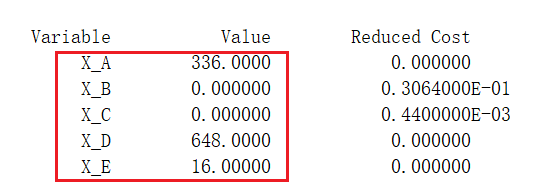
\includegraphics[width=0.7\textwidth]{img/6.png}
\caption{最优解}
\end{figure}

投资需要改变,新的最优解为

\[
\begin{aligned}
    x_A &= 336.0000 \\
    x_B &= 0.000000 \\
    x_C &= 0.000000 \\
    x_D &= 648.0000 \\
    x_E &= 16.00000 \\
\end{aligned}
\]

\section*{问题2}

\subsection*{问题描述}
有 4 名同学到一家公司参加三个阶段的面试。公司要求每个同学都必须首先参加秘书初试,然后到部门主管复试,最后到经理处参加面试,并且不允许插队(即在任何一个阶段 4 名同学的顺序是一样的)。由于 4 名同学的专业背景不同,所以每人在三个阶段的面试时间也不同,如下表所示(单位:分钟):

\[
\begin{array}{|c|c|c|c|}
\hline
\textbf{同学} & \textbf{秘书初试(分钟)} & \textbf{主管复试(分钟)} & \textbf{经理面试(分钟)} \\
\hline
\text{同学 A} & 13 & 15 & 20 \\
\text{同学 B} & 10 & 20 & 18 \\
\text{同学 C} & 20 & 16 & 10 \\
\text{同学 D} & 8 & 10 & 15 \\
\hline
\end{array}
\]

这 4 名同学约定他们全部面试完成后一起离开公司。假定现在时间是早上 8:00,问他们最早何时能离开公司?

\subsection*{{\heiti 解答}}

设二元变量 $x_{ik}$ 表示同学 $i$ 在同学 $k$ 之前面试; $s_{ij}$ 表示同学 $i$ 在第 $j$ 个阶段面试的开始时间; $t_{ij}$ 表示同学 $i$ 在第 $j$ 个阶段面试的结束时间。其中,$i,k = A, B, C, D$; $j = 1, 2, 3$。

该问题的目标为最小化最后一个同学面试结束的时间,即
$$
\min R = \max_i (s_{i3} + t_{i3}), \quad i = A, B, C, D
$$

每位同学只有在完成上一轮面试后才能进行下一轮面试,约束条件为
$$
s_{ij} + t_{ij} \leq s_{ij+1}, \quad i = A, B, C, D, \quad j = 1, 2
$$

对于同一轮面试,同学之间不能插队,约束条件为
$$
\begin{cases}
    s_{ij} + t_{ij} \leq s_{kj}, \quad \text{if } x_{ik} = 1 \\
    s_{kj} + t_{kj} \leq s_{ij}, \quad \text{if } x_{ik} = 0 \\
\end{cases}
$$
移项得
$$
\begin{cases}
    s_{ij} + t_{ij} - s_{kj} \leq 0, \quad \text{if } x_{ik} = 1 \\
    s_{kj} + t_{kj} - s_{ij} \leq 0, \quad \text{if } x_{ik} = 0 \\
\end{cases}
$$
考虑到 $s_{ij} + t_{ij} - s_{kj} \leq s_{ij+1} - s_{kj} \leq R$ 必然成立,因此可以将上述约束条件化为
$$
\begin{cases}
    s_{ij} + t_{ij} - s_{kj} \leq R \cdot (1 - x_{ik}) \\
    s_{kj} + t_{kj} - s_{ij} \leq R \cdot x_{ik} \\
\end{cases}
$$

我们发现,目标函数可以化为线性约束,即
$$
\begin{cases}
    \min R \\
    s_{i3} + t_{i3} \leq R, \quad i = A, B, C, D
\end{cases}
$$

所有约束条件为
$$
\begin{cases}
    R \geq s_{i3} + t_{i3}, \quad i = A, B, C, D \\
    s_{ij} + t_{ij} \leq s_{ij+1}, \quad i = A, B, C, D, \quad j = 1, 2 \\
    s_{ij} + t_{ij} - s_{kj} \leq R \cdot (1 - x_{ik}), \quad i = A, B, C, D, \quad j = 1, 2 \\
    s_{kj} + t_{kj} - s_{ij} \leq R \cdot x_{ik}, \quad i = A, B, C, D, \quad j = 1, 2 \\
    s_{ij} \geq 0, \quad i = A, B, C, D, \quad j = 1, 2, 3 \\
    t_{ij} \geq 0, \quad i = A, B, C, D, \quad j = 1, 2, 3 \\
    x_{ik} \in \{0, 1\}, \quad i = A, B, C, D, \quad k = A, B, C, D
\end{cases}
$$

在 Lingo 中建立模型,求解得到最优解。

\begin{figure}[H]
\centering
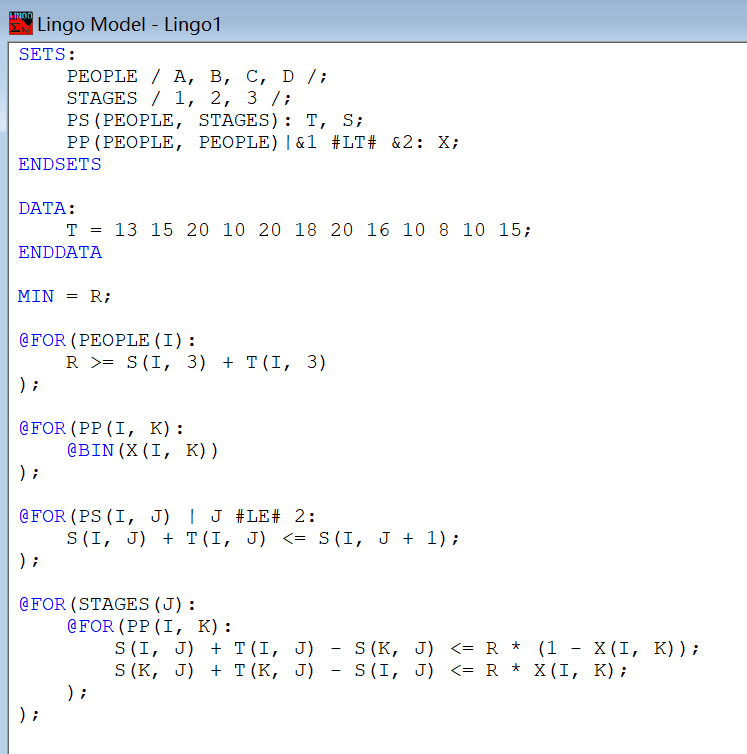
\includegraphics[width=0.9\textwidth]{img/7.png}
\caption{在 Lingo 中建立模型}
\end{figure}

\begin{figure}[H]
\centering
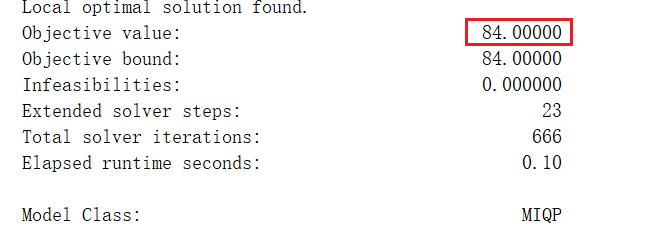
\includegraphics[width=0.5\textwidth]{img/8.png}
\caption{最优解}
\end{figure}

\begin{figure}[H]
\centering
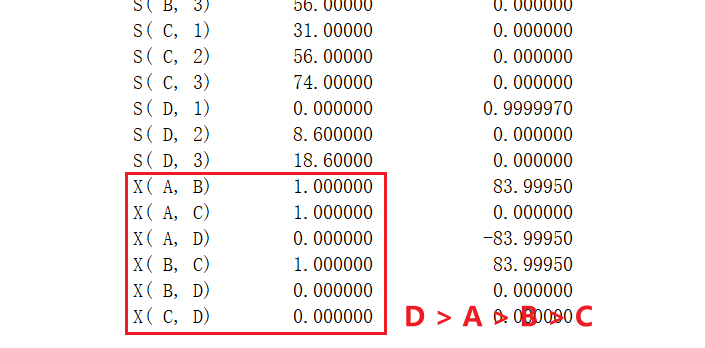
\includegraphics[width=0.7\textwidth]{img/9.png}
\caption{最优解的排序方式}
\end{figure}

最少需要 83 分钟,即 9:23 离开公司。面试的顺序为:同学 D, 同学 A, 同学 B, 同学 C。


\end{document}